%%%%%%%%%%%%%%%%%%
% DOCUMENT CLASS %
%%%%%%%%%%%%%%%%%%
\documentclass{article}

%%%%%%%%%%%%
% PACKAGES %
%%%%%%%%%%%%
\usepackage{hyperref}
\usepackage{graphicx}

%%%%%%%%%%%%%%%%%%
% BEGIN DOCUMENT %
%%%%%%%%%%%%%%%%%%
\begin{document}

%%%%%%%%%
% TITLE %
%%%%%%%%%
\title{Exercise 6}

%%%%%%%%
% DATE %
%%%%%%%%
\date{Due 7/7/2017}

%%%%%%%%%%%%%%
% MAKE TITLE %
%%%%%%%%%%%%%%
\maketitle

\section{Introduction}
This exercise implements the code generation part of compiling StarKist
programs into MIPS assembly. The details of the StarKist programming language
(including its syntax and semantics) were described previously in exercise $5$.
The code generation module traverses the AST built by Bison,
and builds an intermediate representation (IR) tree.
The IR tree is then scanned in a post order fashion
to further translate it into MIPS assembly.
These two phases are summarized in Table \ref{Table_The_Two_Phases_Of_Code_Gen}.
\begin{table}[h]
\centering
\begin{tabular}{ l l}
  Phase$(1)$   & AST $\rightarrow$ IR       \\
  Phase$(2)$   & IR  $\rightarrow$ ASM file \\
\end{tabular}
\caption{
The code generation module can be roughly divided into two phases:
from AST to IR, and then from IR to the actual assembly file.
\label{Table_The_Two_Phases_Of_Code_Gen}}
\end{table}
Note, that different flavours of IR exist, and for example,
gcc alone uses \href{https://gcc.gnu.org/onlinedocs/gccint/Tree-SSA.html#Tree-SSA}
{three kinds of intermediate representations}:\\
\href{https://gcc.gnu.org/onlinedocs/gccint/GENERIC.html#GENERIC}{generic},
\href{https://gcc.gnu.org/onlinedocs/gccint/GIMPLE.html#GIMPLE}{gimple} and
\href{https://gcc.gnu.org/onlinedocs/gccint/RTL.html#RTL}{rtl}.
In our project, we will use a (single) low level IR (LIR),
which is somewhat reminiscent of gcc's
\href{https://gcc.gnu.org/onlinedocs/gccint/RTL.html#RTL}{rtl}.
The term ``low level" here indicates that our IR will contain only a limited set
of commands, specified in Table \ref{Table_IR_API_StarKist}.
Evidently, choosing a low level IR affects the workload between the two phases
mentioned above, and makes for an easier second phase on the expense of
a harder first phase.

\section{IR Specification}
The entire set of IR commands is given in Table \ref{Table_IR_API_StarKist}.
We will briefly describe each of the commands now.
\textbf{BINOP} performs the binary operation between its two sub trees,
the left sub tree is evaluated first.
\textbf{MOVE} stores a source value (sub tree) to a destination which is either a memory address
(\textbf{MEM} sub tree) or a temporary (\textbf{TEMP} sub tree, which is actually a leaf).
The destination is evaluated first.
\textbf{SEQ} indicates a sequence of its two sub trees,
and as before, the left sub tree is evaluated first.
\textbf{CONST} is a leaf containing a single integer as its value.
\textbf{JUMP} and \textbf{LABEL} are (self explanatory) leaves too.
\textbf{CJUMP} evaluates its left and right sub trees in order, 
and conditionally jumps to one of two possible labels
according to the result of the comparison.
\textbf{FUNC} should ideally abstract away both prologue/epilogue
and calling convention, and contain only the signature
of the function and its body.
However, this property is somewhat violated in our project,
and for code readability reasons, the current implementation
contains both prologue/epilogue and the (standard) calling convention.
Note in addition, that unlike most programming languages,
a function in StarKist can \textit{not} return from multiple places,
so there is no need for a \textbf{RET} IR command.

\begin{table}[h]
\centering
\begin{tabular}{ l l l}
  BINOP  & MOVE  & MEM    \\
  CJUMP  & JUMP  & CONST  \\
  LABEL  & TEMP  & CALL   \\
  FUNC   & SEQ   &
\end{tabular}
\caption{
The IR tree nodes.
\label{Table_IR_API_StarKist}}
\end{table}

\section{Inspecting the IR Tree}
To create a graph visualization of the IR tree,
please install graphviz on your machine and run
\[
\verb"$ dot -Tjpeg -o ./IR_Graph.jpeg ./IR_Graph.txt"
\]
from the relevant directory containing the intermediate files.

\section{Running Example}
Consider the simple program in Table \ref{Table_StarKist_Program_Running_Example}.
\begin{table}[h]
\centering
\begin{tabular}{l l}
  let    &                                                   \\
         & type address = $\{$Apt:int, rent:int, ZIP:int$\}$ \\
         & var home:address := address$\{$19, 7500, 6701$\}$ \\
  in     &                                                   \\
         & PrintInt(home\verb"->"ZIP)                    \\
  end    &                                                   \\
\end{tabular}
\caption{
A simple StarKist program that contains one local variable,
one allocation, one field access and one function call.
\label{Table_StarKist_Program_Running_Example}}
\end{table}
It contains a single local variable, a single allocation,
one field access, and one function call.
Note that allocations are done by calling the corresponding
library functions: AllocateRecord and AllocateArray.
The IR tree for this program is shown in Figure \ref{IR_Tree_Running_Example},
and for example, it is immediate to find the variable ``home" there:
\[
\verb"MEM[BINOP(PLUS)(TEMP(fp),-4)]"
\]
An observant reader might also notice that the initializing
fields sent to allocate array are in reverse order.
This is done in order to enable an easier translation
that uses the standard calling convention.
Another point worth mentioning is that allocate record is a
\href{https://en.wikipedia.org/wiki/Variadic_function}{variadic function},
and so the actual number of parameters sent must be passed too.
This is the last CONST$(3)$ in the call to allocate record.
\begin{figure}[htbp]
\begin{center}
  % Requires \usepackage{graphicx}
  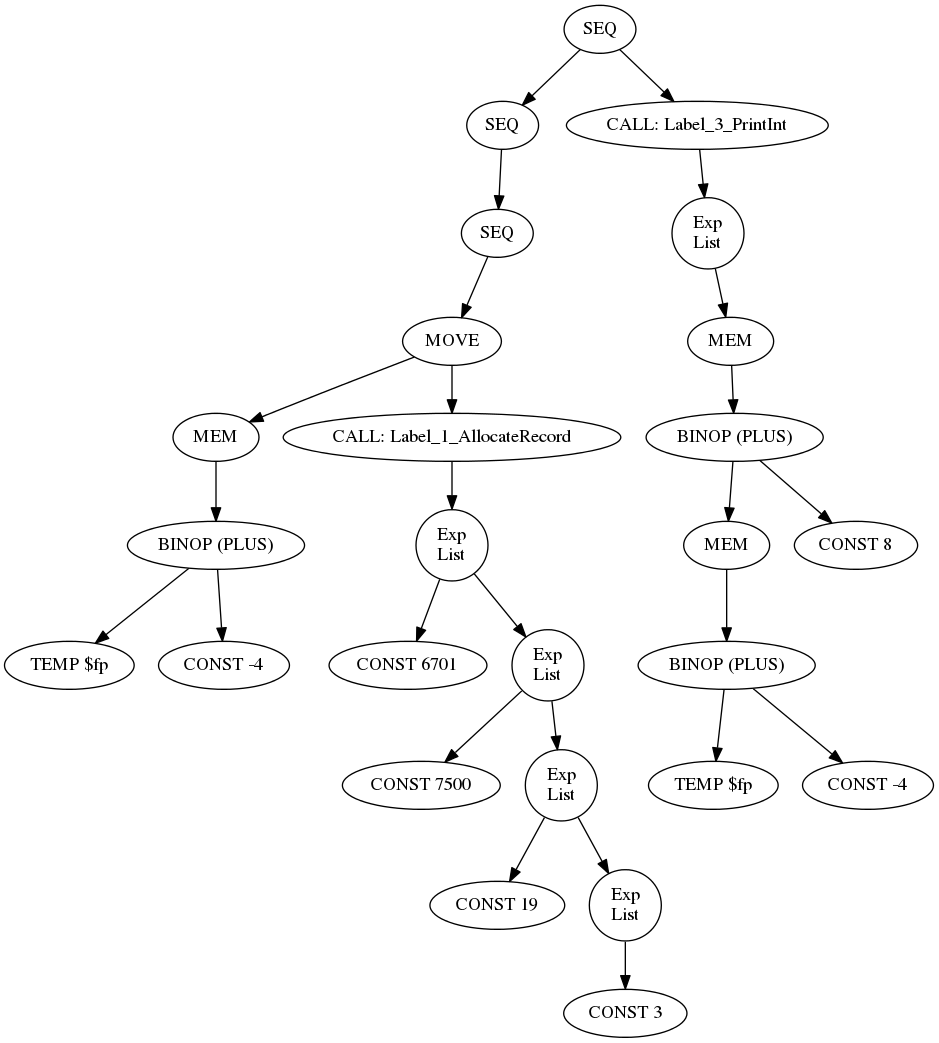
\includegraphics[width = 10cm]{IRTreeRunningExample.png}\\
  \caption{IR tree for the StarKist program in Table \ref{Table_StarKist_Program_Running_Example}.
  \label{IR_Tree_Running_Example}}
\end{center}
\end{figure}

\section{Translation from IR to ASM}
Translation from IR to ASM involves two parts too.
Initially, the IR tree is scanned in a post order fashion,
to produce a pseudo ASM text file with an unbounded number of temporaries.
Then, the register allocation phase replaces those temporaries with
the actual registers of the chosen ASM language. 
These phases are explained thoroughly in class.

\section{Programming Assignment}
Your entire assignment is within the creation of the IR tree.
The translation from IR to MIPS assembly already exists in the code repository.
You will need to implement the runtime mechanism that
checks out of bounds array accesses and null dereferences.
In addition, you will need to implement all the details
to support classes and inheritance
(namely, accessing data members of classes, and virtual function calls) 

\section{Input}
The input for this exercise is a single text file, the input StarKist program.

\section{Output}
The output is a MIPS asm text file that contains the compiled StarKist program.
Currently, the supplied makefile uses (UBUNTU's native MIPS simulator) spim
to run your compiled program and save results in the output directory:
\[
\verb"spim -file compiledProgram.s > Output.txt"
\]
Please make sure that \textit{every} StarKist program given to you does what is expected to do
(printing primes between $2$ and $100$, merging sorted lists, checking out of bound
array accesses etc.)

\section{Submission Guidelines}
The code for this exercise resides as usual in subdirectory EX6 of the course GitHub.
Next, you need to add the relevant derivation rules and AST constructors
for classes. Last, you should implement the missing parts of the Starkist semantic analyzer.
The semantic analyzer resides in the file semant.c, and this is where
most of your changes will occur.
Please submit your exercise in your GitHub repository under COMPILATION/EX6,
and have a makefile there to build a runnable program called compiler.
Make sure that compiler is created in the same level as the makefile: inside EX6.
To avoid the pollution of EX6, please remove all *.o files once the target is built.
The next paragraph describes the execution of compiler.

\paragraph{Execution parameters}
compiler receives $2$ input file names:\\ \\
InputStarkistProgram.txt\\
OutputMipsAsm.s

\end{document}
